\chapter{L'organogenèse~: la construction du membre des tétrapodes}\label{ch:b2:limb-organogenesis}

Trois jours après la ponte d'un œuf de poule, une bosse de la taille
d'une tête d'épingle apparaît sur chaque flanc de l'embryon. Quatre
jours plus tard, c'est une aile, avec un humérus, un radius et un
cubitus, un poignet et trois doigts, dans le bon ordre, de la bonne
longueur, avec des muscles attachés aux bons os. Coupez le liseré de
peau épaissie qui borde la bosse, et l'aile cesse de croître~; greffez
un fragment de son bord postérieur sur son bord antérieur, et elle
développe six doigts disposés en miroir. Le \omterm{def:b2:limb-organogenesis:bud}{bourgeon de membre} est le
cas d'école de l'\emph{organogenèse} --- la construction d'un organe à
partir d'un champ de cellules par des signaux qui indiquent à chaque
cellule à quelle distance elle se trouve de la base, de l'avant et du
dessus --- et les expériences qui l'ont décryptée comptent parmi les plus
limpides de la biologie. Ce chapitre suit le bourgeon depuis sa
croissance jusqu'à son squelette.

\section{Le bourgeon et ses trois axes}

\begin{definition}[Le bourgeon de membre]\label{def:b2:limb-organogenesis:bud}
\index{bourgeon de membre}\index{crete apicale ectodermique@crête apicale ectodermique}\index{zone d'activite polarisante@zone d'activité polarisante}
Le \emph{bourgeon de membre} est un renflement du \emph{mésoderme de la
lame latérale} recouvert d'ectoderme, qui apparaît à une position fixe
le long du flanc (le \emph{champ de membre}) là où le code Hox de l'axe
du corps le permet~; son mésoderme formera les os, le cartilage, les
tendons et le derme, et des cellules venues des somites, qui y
migrent, formeront les muscles. Le bourgeon a trois axes, chacun
gouverné par un centre de signalisation. L'axe \emph{proximo-distal}
(de l'épaule au bout des doigts)~: la \emph{crête apicale ectodermique}
(AER), une bande épaissie d'ectoderme le long de l'extrémité, sécrète
des \omterm{prop:b2:limb-organogenesis:aer}{facteurs de croissance des fibroblastes} (FGF) qui maintiennent le
mésoderme sous-jacent en division et indifférencié. L'axe
\emph{antéro-postérieur} (du pouce à l'auriculaire)~: la \emph{zone
d'activité polarisante} (ZPA), un bloc de mésoderme situé au bord
postérieur, sécrète le morphogène \emph{\omterm{prop:b2:limb-organogenesis:zpa}{Sonic hedgehog}} (Shh). L'axe
\emph{dorso-ventral} (du dos de la main à la paume)~: l'ectoderme dorsal
sécrète Wnt7a. Les bourgeons des membres antérieurs et postérieurs se
ressemblent et utilisent les mêmes signaux~; ils diffèrent par un
facteur de transcription exprimé avant l'apparition du bourgeon (Tbx5
dans le membre antérieur, Tbx4 dans le membre postérieur), et c'est
pourquoi une aile est une aile.
\end{definition}

\begin{omfigure}
\begin{tikzpicture}[every node/.style={font=\scriptsize}, >=stealth]
  % flank
  \fill[omExo!25] (0,-2.2) rectangle (1.2,2.2); \node[rotate=90] at (0.6,0) {paroi du corps (flanc)};
  % bud outline: paddle
  \draw[thick, fill=omDef!10] (1.2,1.4) .. controls (3.0,1.9) and (5.2,1.6) .. (5.8,0.3) .. controls (5.9,-0.3) and (5.2,-1.6) .. (3.4,-1.7) .. controls (2.4,-1.8) and (1.6,-1.5) .. (1.2,-1.4);
  % AER along the tip
  \draw[line width=3pt, omThm] (5.2,1.3) .. controls (5.9,0.6) and (5.9,-0.6) .. (5.0,-1.4);
  \node[omThm, anchor=west, align=left] at (6.1,0.9) {crête apicale ectodermique (AER)~:\\FGF, croissance proximo-distale};
  % ZPA posterior
  \draw[thick, omProp, fill=omProp!50] (2.4,-1.1) ellipse (0.55 and 0.4);
  \draw[omProp] (2.4,-1.5) -- (2.4,-2.0);
  \node[omProp, anchor=north, align=center] at (2.6,-2.0) {ZPA (bord postérieur)~:\\Sonic hedgehog, axe antéro-postérieur};
  % dorsal ectoderm
  \draw[line width=2pt, omDef!70!black] (1.4,1.55) .. controls (3.0,2.0) and (5.0,1.7) .. (5.4,1.2);
  \node[omDef!70!black, anchor=south] at (3.4,2.05) {ectoderme dorsal~: Wnt7a, axe dorso-ventral};
  % axes
  \draw[->, thick] (1.5,-3.1) -- (5.5,-3.1); \node[below] at (3.5,-3.15) {proximal $\to$ distal};
  \draw[->, thick] (10.6,-1.6) -- (10.6,1.2); \node[right, align=left] at (10.7,-0.2) {postérieur $\to$ antérieur\\(de l'auriculaire au pouce)};
\end{tikzpicture}

{\small Le \omterm{def:b2:limb-organogenesis:bud}{bourgeon de membre} du poulet vu de dessus, avec ses trois
centres de signalisation~: l'AER le long de l'extrémité commande la
croissance, la ZPA au bord postérieur organise les doigts, l'ectoderme
dorsal distingue le dos de la paume.}
\end{omfigure}

\begin{omfigure}
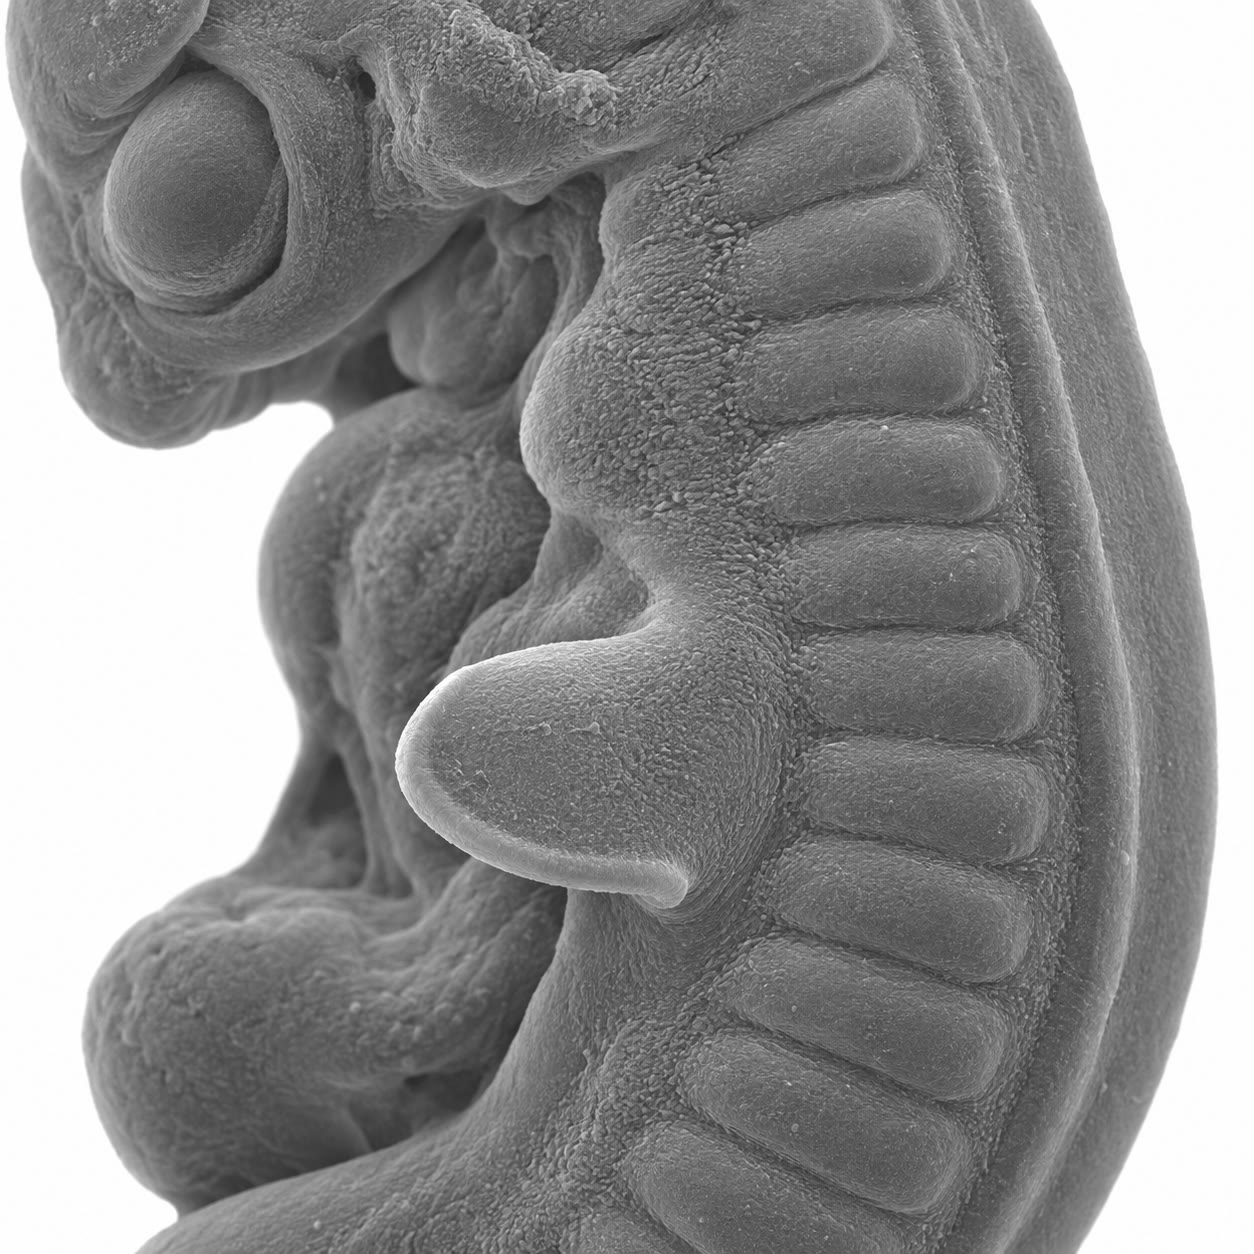
\includegraphics[width=0.42\linewidth]{images/book4/ai/b4-11-limb-bud.jpg}

{\small Un embryon de poulet au microscope électronique à balayage~: la
rangée de somites le long du tronc et, sur le flanc, le \omterm{def:b2:limb-organogenesis:bud}{bourgeon de
membre} en forme de palette, avec la crête épaissie le long de son bord.}
\end{omfigure}

\section{La croissance~: l'axe proximo-distal}

\begin{proposition}[La crête apicale ectodermique]\label{prop:b2:limb-organogenesis:aer}
\index{facteur de croissance des fibroblastes}\index{zone de progression}
L'AER est nécessaire à la croissance, et ses FGF suffisent~: le
mésoderme sous-jacent, la \emph{\omterm{prop:b2:limb-organogenesis:aer}{zone de progression}}, se divise environ
toutes les douze heures, et les cellules qui quittent la zone à mesure
que l'extrémité avance cessent de se diviser, se condensent et se
différencient. Le squelette se forme dans l'ordre proximo-distal ---
\emph{stylopode} (humérus ou fémur), \emph{zeugopode} (radius et
cubitus, tibia et péroné), \emph{autopode} (poignet et doigts) ---
chaque segment étant spécifié à son tour à mesure que le bourgeon croît,
et les segments correspondent à des domaines emboîtés d'expression des
gènes Hox (Hoxa/d 9--10 dans le stylopode, 11 dans le zeugopode, 13 dans
l'autopode). Un \omterm{def:b2:limb-organogenesis:bud}{bourgeon de membre} s'allonge d'un facteur dix environ en
quatre jours, tandis que la portée du signal de la crête reste de
quelques centaines de micromètres~: la crête organise donc le membre
non pas d'un seul coup, mais comme un front mobile, à la manière d'une
imprimante qui trace une page ligne par ligne.
\end{proposition}
\begin{proof}[Faits expérimentaux]
Saunders (1948) retira l'AER de bourgeons d'aile de poulet à des stades
successifs~: retirée tôt, le bourgeon ne donnait qu'un moignon
d'humérus~; retirée un jour plus tard, un humérus et un avant-bras mais
pas de main~; retirée plus tard encore, une aile presque complète ---
plus l'opération est tardive, plus le niveau de troncature est distal~:
la crête est donc nécessaire à chaque segment tour à tour. La greffe
d'une seconde crête produisait une seconde excroissance~; une bille
imbibée de FGF, posée sur un bourgeon dont la crête avait été retirée,
restaurait un membre complet (Niswander, 1993), et une bille placée sur
le flanc entre les champs de membres induisait un membre surnuméraire.
Les souris dépourvues des FGF de la crête n'ont pas de membres.
\end{proof}

\begin{omfigure}
\begin{tikzpicture}[every node/.style={font=\scriptsize}]
  \foreach \x/\lab/\n in {0/{AER retirée tôt~:\\humérus seul}/1, 3.6/{retirée un jour plus tard~:\\humérus, radius, cubitus}/2, 7.2/{retirée plus tard encore~:\\aile presque complète}/3, 10.8/{intacte~:\\aile complète}/4} {
    \begin{scope}[xshift=\x cm]
      \fill[omExo!25] (0,-0.5) rectangle (0.5,2.6);
      % humerus
      \draw[thick, fill=omDef!25, rounded corners=3pt] (0.6,0.9) rectangle (1.7,1.2);
      \ifnum\n>1 \draw[thick, fill=omDef!25, rounded corners=3pt] (1.8,1.05) rectangle (2.7,1.3); \draw[thick, fill=omDef!25, rounded corners=3pt] (1.8,0.75) rectangle (2.7,1.0); \fi
      \ifnum\n>2 \foreach \y in {0.55,0.85,1.15} \draw[thick, fill=omDef!25, rounded corners=2pt] (2.8,\y) rectangle (3.3,\y+0.2); \fi
      \ifnum\n=4 \foreach \y in {0.55,0.85,1.15} \draw[thick, fill=omDef!25, rounded corners=2pt] (3.35,\y) rectangle (3.5,\y+0.2); \fi
      \node[below, align=center] at (1.8,-0.2) {\lab};
    \end{scope}
  }
\end{tikzpicture}

{\small L'expérience de Saunders. Plus la crête est retirée tôt, plus la
partie manquante du membre est grande, toujours à partir de
l'extrémité~: la crête est nécessaire à chaque segment pendant sa mise
en place.}
\end{omfigure}

\begin{theorem}[La croissance par division]\label{thm:b2:limb-organogenesis:growth}
Un bourgeon dont les cellules se divisent toutes les $T$ heures
multiplie son nombre de cellules par $2^{t/T}$ en un temps $t$~; quatre
jours de cycles de douze heures donnent $2^{8} = 256$. Si le volume du
bourgeon est multiplié par mille en ces quatre jours, la division fournit
un facteur 256, et le facteur quatre restant doit venir de
l'agrandissement des cellules et de la matrice que les cellules
cartilagineuses sécrètent autour d'elles. Réciproquement, un segment qui
demande un cycle cellulaire pour être spécifié --- les douze heures
environ qui séparent les niveaux de troncature successifs de
l'expérience de Saunders --- correspond à un doublement de la \omterm{prop:b2:limb-organogenesis:aer}{zone de
progression}.
\end{theorem}
\begin{proof}
$N(t) = N_0 2^{t/T}$~; avec $t = \qty{96}{h}$ et $T = \qty{12}{h}$,
$t/T = 8$. Le rapport du facteur requis au facteur fourni par la
division,
$1000/256 \approx 4$, est ce que doit apporter la croissance autre que
la division.
\end{proof}

\section{Les doigts~: l'axe antéro-postérieur}

\begin{proposition}[La zone d'activité polarisante]\label{prop:b2:limb-organogenesis:zpa}
\index{Sonic hedgehog}\index{morphogene!Shh@morphogène!Shh}
La ZPA spécifie quel doigt se forme où. Ses cellules sécrètent \omterm{prop:b2:limb-organogenesis:zpa}{Sonic
hedgehog}, qui se répand dans le bourgeon à partir du bord postérieur,
et les cellules du mésoderme lisent la concentration --- et la durée
pendant laquelle elles y ont été exposées --- comme une position~: la
dose la plus forte donne le doigt le plus postérieur, des doses plus
faibles des doigts plus antérieurs, et en dessous d'un seuil aucun
doigt. Le gradient a la forme exponentielle vue au
\cref{ch:b2:vertebrate-development}, avec une longueur de décroissance
de quelques dizaines de micromètres, et ses seuils découpent le
bourgeon en ébauches de doigts~: dans l'aile de poulet, du postérieur à
l'antérieur, les doigts 4, 3 et 2. Une seconde source du signal au bord
antérieur produit une seconde série, disposée en miroir~; une source
plus faible, ou une exposition plus courte, ne produit que les doigts
antérieurs de la série surnuméraire. Le même gène, dans le même rôle,
organise les doigts de tous les tétrapodes, et une \omterm{def:b2:genome-diversification:mutation}{mutation} qui ajoute
une source antérieure de Shh donne une polydactylie chez le chat, le
poulet, la souris et l'être humain.
\end{proposition}
\begin{proof}[Faits expérimentaux]
Saunders et Gasseling (1968) greffèrent un bloc de mésoderme du bord
postérieur d'un bourgeon d'aile de poulet sur le bord antérieur d'un
autre~: l'hôte développa une aile à six doigts dans l'ordre 4-3-2-2-3-4,
image en miroir de part et d'autre du milieu. Tickle (1975) montra que
le nombre de doigts surnuméraires dépendait du nombre de cellules
greffées --- une dose. Riddle et Tabin (1993) découvrirent que le tissu
greffé exprimait le gène \emph{\omterm{prop:b2:limb-organogenesis:zpa}{Sonic hedgehog}}, que ce gène n'était
exprimé nulle part ailleurs dans le bourgeon, et que des cellules
modifiées pour l'exprimer, greffées en position antérieure,
reproduisaient la duplication en miroir~; une bille imbibée de la
protéine produisait le même effet. Les poulets mutants porteurs d'une
tache ectopique antérieure de Shh ont des doigts antérieurs
surnuméraires.
\end{proof}

\begin{omfigure}
\begin{tikzpicture}[every node/.style={font=\scriptsize}, >=stealth]
  % normal bud with gradient and digits
  \begin{scope}
    \fill[omExo!25] (0,-0.3) rectangle (0.4,3.3);
    \shade[bottom color=omProp!60, top color=white] (0.4,-0.3) rectangle (3.2,3.3);
    \draw[thick] (0.4,-0.3) rectangle (3.2,3.3);
    \draw[thick, omProp, fill=omProp!70] (0.9,0.1) ellipse (0.45 and 0.35); \node[omProp!80!black, anchor=west] at (1.4,0.1) {ZPA};
    \foreach \y/\d in {0.6/4, 1.5/3, 2.4/2} { \draw[thick, fill=omDef!25, rounded corners=2pt] (3.3,\y-0.12) rectangle (4.2,\y+0.12); \node[right] at (4.25,\y) {doigt \d}; }
    \node[below, align=center] at (2.0,-0.5) {bourgeon normal~: Shh issu du\\bord postérieur, doigts 4-3-2};
    \draw[->, thick] (-0.4,0.2) -- (-0.4,3.0); \node[rotate=90] at (-0.7,1.6) {postérieur $\to$ antérieur};
  \end{scope}
  % grafted bud
  \begin{scope}[xshift=7cm]
    \fill[omExo!25] (0,-0.3) rectangle (0.4,3.3);
    \shade[bottom color=omProp!60, top color=white] (0.4,-0.3) rectangle (3.2,1.5);
    \shade[top color=omProp!60, bottom color=white] (0.4,1.5) rectangle (3.2,3.3);
    \draw[thick] (0.4,-0.3) rectangle (3.2,3.3);
    \draw[thick, omProp, fill=omProp!70] (0.9,0.1) ellipse (0.45 and 0.35);
    \draw[thick, omProp, fill=omProp!70] (0.9,2.9) ellipse (0.45 and 0.35); \node[omProp!80!black, anchor=west] at (1.4,2.9) {ZPA greffée};
    \foreach \y/\d in {0.3/4, 0.8/3, 1.3/2, 1.7/2, 2.2/3, 2.7/4} { \draw[thick, fill=omDef!25, rounded corners=2pt] (3.3,\y-0.1) rectangle (4.2,\y+0.1); \node[right] at (4.25,\y) {\d}; }
    \node[below, align=center] at (2.0,-0.5) {ZPA greffée en avant~:\\duplication en miroir 4-3-2-2-3-4};
  \end{scope}
\end{tikzpicture}

{\small La région polarisante. À gauche~: Shh se répand à partir du bord
postérieur, et sa concentration décroissante spécifie les doigts 4, 3
et 2. À droite~: une seconde ZPA greffée sur le bord antérieur crée un
second gradient et une série de doigts disposée en miroir.}
\end{omfigure}

\begin{theorem}[Les frontières des doigts à partir du gradient]\label{thm:b2:limb-organogenesis:thresholds}
Avec Shh à la concentration $c_0$ au bord postérieur et une longueur de
décroissance $\lambda$, la frontière du territoire d'un doigt de seuil
$T_i$ se situe à $x_i = \lambda\ln(c_0/T_i)$ du bord. Avec
$\lambda = \qty{50}{\micro m}$ et des seuils de $0.6$,
$0.25$ et $0.08$ de $c_0$ pour les doigts 4, 3 et 2, les territoires
s'étendent de $0$ à $26$, de $26$ à $69$ et de $69$ à $126$ micromètres,
et le tissu situé au-delà de \qty{126}{\micro m} ne forme aucun doigt.
Doubler la source déplace chaque frontière vers l'extérieur de
$\lambda\ln 2 = \qty{35}{\micro m}$
--- assez, dans un bourgeon de quelques centaines de micromètres, pour
ajouter un doigt au bord antérieur~; une seconde source au bord
antérieur dispose les mêmes territoires en sens inverse.
\end{theorem}
\begin{proof}
D'après $c(x) = c_0 e^{-x/\lambda}$, $c = T_i$ en $x_i = \lambda
\ln(c_0/T_i)$~: $50\ln(1/0.6) = 25.5$, $50\ln 4 = 69$, $50\ln 12.5 =
126$. Remplacer $c_0$ par $2c_0$ ajoute $\lambda\ln 2$ à chaque $x_i$.
\end{proof}

\begin{omfigure}
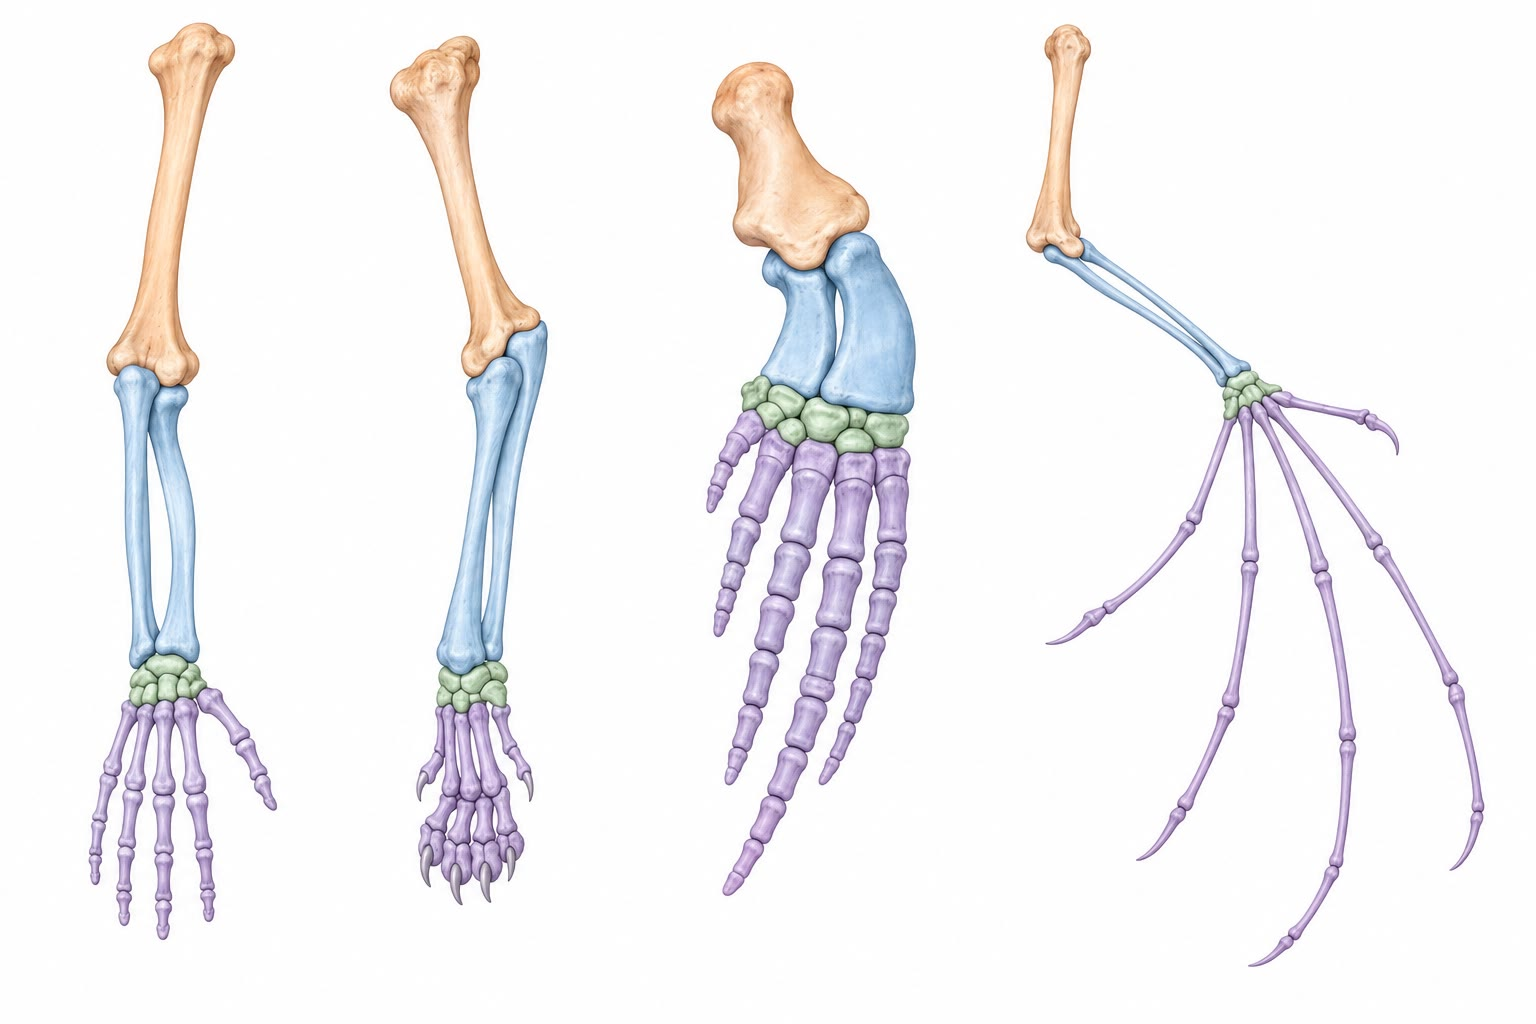
\includegraphics[width=0.66\linewidth]{images/book4/ai/b4-11-tetrapod-limbs.jpg}

{\small Un plan, quatre membres~: les membres antérieurs d'un être
humain, d'un chat, d'une baleine et d'une chauve-souris partagent les
mêmes os dans le même ordre --- un stylopode, deux os du zeugopode, un
poignet, des doigts --- construits par les mêmes centres de
signalisation et différant par leur croissance.}
\end{omfigure}

\section{Coordination et modelage}

\begin{proposition}[Les axes dialoguent]\label{prop:b2:limb-organogenesis:loop}
\index{boucle de retroaction!du developpement@boucle de rétroaction!du développement}
Les centres s'entretiennent mutuellement~: le FGF de la crête maintient
l'expression de Shh par la ZPA, et Shh, par un relais dans le
mésoderme, maintient l'expression de FGF par la crête~; si l'on retire
l'un, l'autre s'éteint en une journée. Wnt7a, issu de l'ectoderme
dorsal, est lui aussi nécessaire à la pleine expression de Shh, et il
impose le destin dorsal du mésoderme (une souris qui en est dépourvue a
deux paumes). Cette dépendance mutuelle est une \emph{boucle de
rétroaction positive} qui verrouille les trois axes ensemble~: le membre
ne croît que là où il est organisé, et n'est organisé que là où il
croît, si bien qu'un bourgeon ne fait jamais une main sans bras ni des
doigts de la mauvaise sorte. Lorsque la croissance est achevée, la
boucle se rompt --- le mésoderme cesse de relayer, Shh s'arrête, la
crête régresse --- et le membre cesse de croître à sa taille normale.
\end{proposition}

\begin{proposition}[Du plan à l'os]\label{prop:b2:limb-organogenesis:skeleton}
\index{chondrogenese@chondrogenèse}\index{apoptose!interdigitale}
Une fois spécifiées, les cellules du mésoderme qui quittent la \omterm{prop:b2:limb-organogenesis:aer}{zone de
progression} se \emph{condensent} en baguettes et en plaques ayant la
forme des futurs os, se différencient en cellules cartilagineuses qui
sécrètent une matrice riche en collagène et en protéoglycanes, et
édifient une maquette cartilagineuse de chaque élément du squelette~;
les articulations se forment là où une bande de cellules reçoit
l'ordre de ne pas devenir du cartilage~; des vaisseaux sanguins envahissent
les maquettes et l'os remplace le cartilage du centre vers la
périphérie, en laissant aux extrémités des cartilages de croissance qui
font s'allonger l'os jusqu'à l'âge adulte (\emph{ossification
endochondrale}). Des précurseurs musculaires issus des somites migrent
dans le membre, se divisent, fusionnent en fibres
(\cref{ch:b2:cell-differentiation}) et s'attachent par des tendons
formés par le mésoderme propre du membre. Entre les rayons des doigts,
le tissu est éliminé par mort cellulaire programmée~: les cellules des
palmures interdigitales, sous l'effet d'un signal de protéine
morphogénétique osseuse (BMP), déclenchent leur propre destruction et
sont éliminées en un jour, ce qui sépare les doigts. Le canard garde ses
palmures parce qu'un inhibiteur de BMP est exprimé dans son tissu
interdigital~; un poulet auquel on applique le même inhibiteur sur une
bille développe des pattes palmées.
\end{proposition}
\begin{proof}[Faits expérimentaux]
Du mésoderme interdigital prélevé sur un bourgeon de patte de poulet et
greffé ailleurs meurt au moment prévu --- la mort est intrinsèque,
décidée avant le prélèvement du tissu~; le même tissu prélevé chez le
canard survit. Des billes de BMP placées entre les doigts d'un canard
font mourir la palmure~; des billes de l'inhibiteur gremlin placées
entre les doigts d'un poulet la préservent. Une souris dépourvue d'un
récepteur des BMP dans le membre garde ses palmures.
\end{proof}

\begin{omfigure}
\begin{tikzpicture}[every node/.style={font=\scriptsize}]
  \foreach \x/\lab in {0/{les rayons des doigts se\\condensent en cartilage}, 4.2/{les cellules interdigitales\\meurent (BMP)}, 8.4/{doigts séparés~;\\l'os remplace le cartilage}} {
    \begin{scope}[xshift=\x cm]
      \node[below, align=center] at (1.5,-0.3) {\lab};
    \end{scope}
  }
  % stage 1: paddle with rays
  \draw[thick, fill=omDef!8] (0,0) .. controls (0,2.2) and (3,2.2) .. (3,0) -- cycle;
  \foreach \x in {0.6,1.2,1.8,2.4} \draw[thick, fill=omDef!30, rounded corners=2pt] (\x-0.12,0.1) rectangle (\x+0.12,1.5);
  % stage 2: paddle with dying webs
  \begin{scope}[xshift=4.2cm]
    \draw[thick, fill=omDef!8] (0,0) .. controls (0,2.2) and (3,2.2) .. (3,0) -- cycle;
    \foreach \x in {0.6,1.2,1.8,2.4} \draw[thick, fill=omDef!30, rounded corners=2pt] (\x-0.12,0.1) rectangle (\x+0.12,1.5);
    \foreach \x in {0.9,1.5,2.1} \foreach \y in {0.7,1.0,1.3} \fill[omThm] (\x,\y) circle (0.05);
  \end{scope}
  % stage 3: separated digits
  \begin{scope}[xshift=8.4cm]
    \draw[thick, fill=omDef!8] (0,0) -- (0,0.5) -- (0.3,0.5) -- (0.35,1.7) -- (0.85,1.7) -- (0.9,0.5) -- (1.05,0.5) -- (1.1,1.85) -- (1.6,1.85) -- (1.65,0.5) -- (1.8,0.5) -- (1.85,1.7) -- (2.35,1.7) -- (2.4,0.5) -- (2.7,0.5) -- (2.7,0) -- cycle;
    \foreach \x in {0.6,1.35,2.1} \draw[thick, fill=omExo!60, rounded corners=2pt] (\x-0.1,0.1) rectangle (\x+0.1,1.4);
  \end{scope}
\end{tikzpicture}

{\small Le modelage de la main~: des rayons cartilagineux se condensent
dans la palette, les cellules situées entre eux meurent (en rouge), et
les doigts libérés s'ossifient.}
\end{omfigure}

\begin{example}[Le même membre, autrement développé]\label{ex:b2:limb-organogenesis:evolution}
L'aile de la chauve-souris est une main dont les doigts 2 à 5 ont grandi
plusieurs fois plus que ceux d'une souris --- un amplificateur d'un
gène du membre, transplanté de la chauve-souris à la souris, allonge les
os du membre antérieur de la souris --- et dont le tissu interdigital a
survécu, parce que la palmure exprime l'inhibiteur de BMP qu'utilise le
canard. La nageoire de la baleine est une main pourvue de phalanges
surnuméraires et sans mort interdigitale. La patte du cheval est un
doigt unique, les autres étant réduits à des stylets. Le serpent n'a pas
de membres parce que son flanc n'exprime jamais les signaux qui
déclenchent un bourgeon. Et les nageoires des poissons, dépourvues
d'autopode, sont construites par les mêmes AER et ZPA, mais arrêtent
leur programme Hox avant la phase tardive qui forme les doigts~; le
fossile \emph{Tiktaalik} (375 millions d'années) montre le poignet
apparaissant dans une nageoire. L'évolution des membres consiste
surtout à moduler un programme conservé --- la durée de chaque phase, la
portée de chaque signal, les cellules qui meurent.
\end{example}

\section{Exercices}

\begin{exercise}[$\star$]\label{exo:b2:limb-organogenesis:1}
Nommer les trois axes du \omterm{def:b2:limb-organogenesis:bud}{bourgeon de membre} et, pour chacun, le centre
de signalisation, sa position et son signal.
\end{exercise}

\begin{exercise}[$\star$]\label{exo:b2:limb-organogenesis:2}
Donner les trois segments du squelette du membre et les os de chacun
dans le bras et la jambe humains. Quels gènes Hox les marquent~?
\end{exercise}

\begin{exercise}[$\star$]\label{exo:b2:limb-organogenesis:3}
Énumérer, dans l'ordre, les étapes qui mènent d'une plage de mésoderme
de la lame latérale à un doigt pourvu de son os, de son articulation et
de son muscle.
\end{exercise}

\begin{exercise}[$\star$]\label{exo:b2:limb-organogenesis:4}
À quoi ressemble le membre si l'AER est retirée (a) dès l'apparition du
bourgeon, (b) après la spécification de l'avant-bras, (c) jamais, mais
remplacée par une bille de FGF~?
\end{exercise}

\begin{exercise}[$\star\star$]\label{exo:b2:limb-organogenesis:5}
Avec $\lambda = \qty{40}{\micro m}$ et des seuils de $0.5$, $0.2$
et $0.05$ de la concentration de la source pour les doigts 4, 3 et 2,
calculer les trois frontières et la largeur de chaque territoire de
doigt.
\end{exercise}

\begin{exercise}[$\star\star$]\label{exo:b2:limb-organogenesis:6}
Prévoir la disposition des doigts d'une aile de poulet après (a) la
greffe d'une ZPA entière sur le bord antérieur, (b) la greffe de quatre
fois moins de cellules de ZPA, (c) une bille de Shh posée sur le bord
antérieur et retirée après une courte exposition. Expliquer chaque cas
par la dose et la durée.
\end{exercise}

\begin{exercise}[$\star\star$]\label{exo:b2:limb-organogenesis:7}
Un \omterm{def:b2:limb-organogenesis:bud}{bourgeon de membre} de poulet compte \num{5000} cellules lorsque la
crête se forme, et ses cellules se divisent toutes les \qty{12}{h}.
Combien de cellules au bout de quatre jours~? Si le membre compte à ce
stade $4\times 10^{6}$ cellules, que doit-on en conclure sur le cycle
cellulaire ou sur la mort cellulaire~?
\end{exercise}

\begin{exercise}[$\star\star$]\label{exo:b2:limb-organogenesis:8}
Expliquer pourquoi le poulet a des doigts libres et le canard des pattes
palmées, et ce que produit une bille d'inhibiteur de BMP placée entre
les doigts d'un embryon de poulet. Qu'indique le caractère intrinsèque
du calendrier de la mort interdigitale (elle se produit à l'heure dans
une greffe) sur la manière dont les cellules ont été instruites~?
\end{exercise}

\begin{exercise}[$\star\star$]\label{exo:b2:limb-organogenesis:9}
Une souris est dépourvue à la fois de Hoxa13 et de Hoxd13~; une autre de
Hoxa11 et de Hoxd11. Prévoir le squelette du membre antérieur de chacune
et dire ce que le résultat montre sur la relation entre domaines Hox et
segments.
\end{exercise}

\begin{exercise}[$\star\star\star$]\label{exo:b2:limb-organogenesis:10}
Expliquer la rétroaction positive entre l'AER et la ZPA, pourquoi elle
rend le membre robuste, et ce qui arriverait à un bourgeon dans lequel
Shh ne pourrait pas maintenir le FGF. La comparer à la rétroaction
positive du travail de l'accouchement vue au
\cref{ch:b2:mammal-reproduction}~: qu'est-ce qui met fin à chaque
boucle~?
\end{exercise}

\begin{exercise}[$\star\star\star$]\label{exo:b2:limb-organogenesis:11}
Le troisième doigt d'une chauve-souris est huit fois plus long que
celui d'une souris, rapporté à la taille du corps. Si le cartilage des
doigts s'allonge exponentiellement au taux $r$ par jour pendant une
fenêtre de croissance, et que la fenêtre de la chauve-souris dure quatre
jours de plus que celle de la souris, quel $r$ faut-il~? Donner deux
modifications du développement (l'une de la croissance, l'autre de la
mort cellulaire) qui font d'une main une aile.
\end{exercise}

\begin{exercise}[$\star\star\star$]\label{exo:b2:limb-organogenesis:12}
\omterm{prop:b2:limb-organogenesis:zpa}{Sonic hedgehog} organise le \omterm{prop:b2:vertebrate-development:neurulation}{tube neural} à partir de la plaque du plancher
(\cref{ch:b2:vertebrate-development}) et les doigts à partir de la ZPA.
Discuter pourquoi l'évolution réutilise quelques signaux pour de
nombreuses tâches, comment une même molécule peut avoir des
significations différentes dans des tissus différents, et ce que cela
implique pour l'effet d'une \omterm{def:b2:genome-diversification:mutation}{mutation} d'un tel gène.
\end{exercise}

\section{Problème~: une aile construite en une semaine}

\begin{problem}[{Problème du week-end --- l'aile de poulet suivie du
bourgeon au squelette~: sa croissance par division, le calendrier des
ablations de crête de Saunders, le calcul du gradient de Shh et la
prévision de ses duplications, le modelage des palmures et la
comparaison avec une chauve-souris, jusqu'au nombre de doublements, aux
frontières des doigts et à la largeur qu'exige une duplication en
miroir}]
\label{pb:b2:limb-organogenesis:1}
Un bourgeon d'aile de poulet apparaît au 3\textsuperscript{e} jour
d'incubation, avec \num{2000} cellules mésodermiques et une longueur de
\qty{0.4}{mm}~; au 7\textsuperscript{e} jour, l'aile mesure
\qty{4}{mm} et son volume vaut \num{1000} fois celui du bourgeon. Les
cellules de la \omterm{prop:b2:limb-organogenesis:aer}{zone de progression} se divisent toutes les \qty{12}{h}.
Ablations de la crête~: à 3.0 jours, le membre est un moignon~; à
3.5 jours, un humérus seul~; à 4.0 jours, humérus, radius et cubitus~;
à 4.5 jours, une aile à laquelle ne manquent que les extrémités des
doigts. Shh~: $D = \qty{1e-12}{m^2/s}$, demi-vie \qty{29}{min}~; seuils
$0.6$, $0.25$, $0.08$ de $c_0$ pour les doigts 4, 3, 2. Largeur du
bourgeon (du postérieur à l'antérieur) \qty{600}{\micro m}. Palmures
interdigitales~: trois régions de
\qty{300}{\micro m}$\times$\qty{300}{\micro m}$\times$\qty{200}{\micro m},
cellules de \qty{1000}{\micro m^3}, éliminées en \qty{24}{h}.

\medskip
\noindent\textbf{Partie I --- La croissance.}
\begin{enumerate}
  \item Combien de doublements ont lieu en quatre jours~? Combien de
        cellules cela donne-t-il à partir de \num{2000}~?
  \item Comparer à l'augmentation d'un facteur mille du volume~: quel
        facteur doivent fournir l'agrandissement des cellules et la
        matrice~?
  \item De quel facteur la longueur a-t-elle augmenté~? Si le bourgeon
        croissait comme un cylindre de rayon constant, quel facteur de
        volume cela donnerait-il, et qu'indique la différence sur la
        forme~?
  \item Le FGF de la crête pénètre à \qty{300}{\micro m} dans le
        mésoderme. Quelle fraction du bourgeon est sous son influence au
        3\textsuperscript{e} jour et au 7\textsuperscript{e} jour~?
  \item Expliquer pourquoi un signal de portée fixe dans un organe en
        croissance produit une séquence proximo-distale.
  \item Une cellule quitte la \omterm{prop:b2:limb-organogenesis:aer}{zone de progression} au
        4\textsuperscript{e} jour. À quel segment se joint-elle~?
\end{enumerate}

\medskip
\noindent\textbf{Partie II --- Le calendrier des segments.}
\begin{enumerate}[resume]
  \item D'après la série d'ablations, donner le moment auquel chaque
        segment (stylopode, zeugopode, autopode) a été spécifié.
  \item Combien de cycles cellulaires séparent la spécification de
        segments successifs~?
  \item Expliquer ce résultat en termes de \omterm{prop:b2:limb-organogenesis:aer}{zone de progression} et de
        domaines Hox.
  \item Une bille de FGF est placée sur un bourgeon dont la crête a été
        retirée à 3.5 jours. Prévoir le membre.
  \item Une seconde crête est greffée sur la face dorsale d'un bourgeon
        intact à 3.5 jours. Prévoir le résultat.
  \item Pourquoi le bourgeon cesse-t-il de croître au
        7\textsuperscript{e} jour au lieu de continuer indéfiniment~?
\end{enumerate}

\medskip
\noindent\textbf{Partie III --- Le gradient.}
\begin{enumerate}[resume]
  \item Calculer $k$ et $\lambda$ pour Shh.
  \item Calculer les trois frontières des doigts et les largeurs des
        territoires.
  \item Quelle est la largeur de la région antérieure qui ne forme aucun
        doigt dans un bourgeon de \qty{600}{\micro m}~?
  \item Une \omterm{def:b2:genome-diversification:mutation}{mutation} double la production de Shh. Recalculer les
        frontières et dire si un doigt surnuméraire se forme, et lequel.
  \item Une ZPA est greffée sur le bord antérieur. Quelle largeur
        minimale du bourgeon permet une série complète en miroir
        4-3-2-2-3-4 sans chevauchement des deux territoires du doigt 2~?
        Le bourgeon de poulet est-il assez large~?
  \item Prévoir la disposition si le bourgeon ne mesurait que
        \qty{200}{\micro m} de large.
  \item Pourquoi une greffe d'un quart de la ZPA ne donne-t-elle que
        2-2-3-4~?
\end{enumerate}

\medskip
\noindent\textbf{Partie IV --- Modelage et évolution.}
\begin{enumerate}[resume]
  \item Calculer le nombre de cellules des trois palmures et le rythme
        de la mort cellulaire pendant leur élimination, en cellules par
        seconde.
  \item Les cellules interdigitales du canard expriment un inhibiteur de
        BMP. Prévoir l'effet d'une bille de BMP dans une palmure de
        canard et de l'inhibiteur dans une palmure de poulet.
  \item Le cartilage des doigts d'une chauve-souris croît pendant quatre
        jours supplémentaires à un taux exponentiel de \qty{0.5}{d^{-1}}.
        De quel facteur est-il plus long que celui du poulet~? Nommer une
        seconde modification qui forme la membrane de l'aile.
  \item Un bourgeon de nageoire de poisson possède une AER et une ZPA,
        mais pas de doigts. Que lui manque-t-il, et que montre
        \emph{Tiktaalik}~?
  \item Si les cellules des palmures avaient au contraire été produites
        par division à partir de \num{1000} fondatrices, à raison de
        \qty{12}{h} par cycle, combien de temps leur fabrication
        aurait-elle pris~? Comparer à la journée nécessaire pour les
        éliminer.
  \item Énoncer le résultat~: le nombre de doublements en quatre jours,
        les trois frontières des doigts et la largeur minimale pour une
        duplication en miroir.
\end{enumerate}
\end{problem}
